% Options for packages loaded elsewhere
\PassOptionsToPackage{unicode}{hyperref}
\PassOptionsToPackage{hyphens}{url}
\PassOptionsToPackage{dvipsnames,svgnames,x11names}{xcolor}
%
\documentclass[
  letterpaper,
  DIV=11,
  numbers=noendperiod]{scrartcl}

\usepackage{amsmath,amssymb}
\usepackage{iftex}
\ifPDFTeX
  \usepackage[T1]{fontenc}
  \usepackage[utf8]{inputenc}
  \usepackage{textcomp} % provide euro and other symbols
\else % if luatex or xetex
  \usepackage{unicode-math}
  \defaultfontfeatures{Scale=MatchLowercase}
  \defaultfontfeatures[\rmfamily]{Ligatures=TeX,Scale=1}
\fi
\usepackage{lmodern}
\ifPDFTeX\else  
    % xetex/luatex font selection
\fi
% Use upquote if available, for straight quotes in verbatim environments
\IfFileExists{upquote.sty}{\usepackage{upquote}}{}
\IfFileExists{microtype.sty}{% use microtype if available
  \usepackage[]{microtype}
  \UseMicrotypeSet[protrusion]{basicmath} % disable protrusion for tt fonts
}{}
\makeatletter
\@ifundefined{KOMAClassName}{% if non-KOMA class
  \IfFileExists{parskip.sty}{%
    \usepackage{parskip}
  }{% else
    \setlength{\parindent}{0pt}
    \setlength{\parskip}{6pt plus 2pt minus 1pt}}
}{% if KOMA class
  \KOMAoptions{parskip=half}}
\makeatother
\usepackage{xcolor}
\usepackage[inner=2cm,outer=3cm,top=2cm,bottom=2.5cm]{geometry}
\setlength{\emergencystretch}{3em} % prevent overfull lines
\setcounter{secnumdepth}{3}
% Make \paragraph and \subparagraph free-standing
\makeatletter
\ifx\paragraph\undefined\else
  \let\oldparagraph\paragraph
  \renewcommand{\paragraph}{
    \@ifstar
      \xxxParagraphStar
      \xxxParagraphNoStar
  }
  \newcommand{\xxxParagraphStar}[1]{\oldparagraph*{#1}\mbox{}}
  \newcommand{\xxxParagraphNoStar}[1]{\oldparagraph{#1}\mbox{}}
\fi
\ifx\subparagraph\undefined\else
  \let\oldsubparagraph\subparagraph
  \renewcommand{\subparagraph}{
    \@ifstar
      \xxxSubParagraphStar
      \xxxSubParagraphNoStar
  }
  \newcommand{\xxxSubParagraphStar}[1]{\oldsubparagraph*{#1}\mbox{}}
  \newcommand{\xxxSubParagraphNoStar}[1]{\oldsubparagraph{#1}\mbox{}}
\fi
\makeatother


\providecommand{\tightlist}{%
  \setlength{\itemsep}{0pt}\setlength{\parskip}{0pt}}\usepackage{longtable,booktabs,array}
\usepackage{calc} % for calculating minipage widths
% Correct order of tables after \paragraph or \subparagraph
\usepackage{etoolbox}
\makeatletter
\patchcmd\longtable{\par}{\if@noskipsec\mbox{}\fi\par}{}{}
\makeatother
% Allow footnotes in longtable head/foot
\IfFileExists{footnotehyper.sty}{\usepackage{footnotehyper}}{\usepackage{footnote}}
\makesavenoteenv{longtable}
\usepackage{graphicx}
\makeatletter
\newsavebox\pandoc@box
\newcommand*\pandocbounded[1]{% scales image to fit in text height/width
  \sbox\pandoc@box{#1}%
  \Gscale@div\@tempa{\textheight}{\dimexpr\ht\pandoc@box+\dp\pandoc@box\relax}%
  \Gscale@div\@tempb{\linewidth}{\wd\pandoc@box}%
  \ifdim\@tempb\p@<\@tempa\p@\let\@tempa\@tempb\fi% select the smaller of both
  \ifdim\@tempa\p@<\p@\scalebox{\@tempa}{\usebox\pandoc@box}%
  \else\usebox{\pandoc@box}%
  \fi%
}
% Set default figure placement to htbp
\def\fps@figure{htbp}
\makeatother
% definitions for citeproc citations
\NewDocumentCommand\citeproctext{}{}
\NewDocumentCommand\citeproc{mm}{%
  \begingroup\def\citeproctext{#2}\cite{#1}\endgroup}
\makeatletter
 % allow citations to break across lines
 \let\@cite@ofmt\@firstofone
 % avoid brackets around text for \cite:
 \def\@biblabel#1{}
 \def\@cite#1#2{{#1\if@tempswa , #2\fi}}
\makeatother
\newlength{\cslhangindent}
\setlength{\cslhangindent}{1.5em}
\newlength{\csllabelwidth}
\setlength{\csllabelwidth}{3em}
\newenvironment{CSLReferences}[2] % #1 hanging-indent, #2 entry-spacing
 {\begin{list}{}{%
  \setlength{\itemindent}{0pt}
  \setlength{\leftmargin}{0pt}
  \setlength{\parsep}{0pt}
  % turn on hanging indent if param 1 is 1
  \ifodd #1
   \setlength{\leftmargin}{\cslhangindent}
   \setlength{\itemindent}{-1\cslhangindent}
  \fi
  % set entry spacing
  \setlength{\itemsep}{#2\baselineskip}}}
 {\end{list}}
\usepackage{calc}
\newcommand{\CSLBlock}[1]{\hfill\break\parbox[t]{\linewidth}{\strut\ignorespaces#1\strut}}
\newcommand{\CSLLeftMargin}[1]{\parbox[t]{\csllabelwidth}{\strut#1\strut}}
\newcommand{\CSLRightInline}[1]{\parbox[t]{\linewidth - \csllabelwidth}{\strut#1\strut}}
\newcommand{\CSLIndent}[1]{\hspace{\cslhangindent}#1}

\usepackage{booktabs}
\usepackage{longtable}
\usepackage{array}
\usepackage{multirow}
\usepackage{wrapfig}
\usepackage{float}
\usepackage{colortbl}
\usepackage{pdflscape}
\usepackage{tabu}
\usepackage{threeparttable}
\usepackage{threeparttablex}
\usepackage[normalem]{ulem}
\usepackage{makecell}
\usepackage{xcolor}
\usepackage{longtable}
\usepackage{amsmath}
\usepackage{amssymb}
\usepackage{multicol}
\usepackage{float}
\usepackage{typearea}
\floatplacement{figure}{htbp}
\floatplacement{table}{htbp}
\AtBeginDocument{%
  \storeareas\normalpapersize
}
\BeforeRestoreareas{\cleardoublepage}
\newcommand*\uselandscape{%
  \cleardoublepage
  \KOMAoptions{paper=landscape}%
  \recalctypearea
  \areaset{1.2\textwidth}{1.2\textheight}%
}
\renewcommand*{\thesection}{S\arabic{section}}
\KOMAoption{captions}{tableheading}
\makeatletter
\@ifpackageloaded{caption}{}{\usepackage{caption}}
\AtBeginDocument{%
\ifdefined\contentsname
  \renewcommand*\contentsname{Table of contents}
\else
  \newcommand\contentsname{Table of contents}
\fi
\ifdefined\listfigurename
  \renewcommand*\listfigurename{List of Figures}
\else
  \newcommand\listfigurename{List of Figures}
\fi
\ifdefined\listtablename
  \renewcommand*\listtablename{List of Tables}
\else
  \newcommand\listtablename{List of Tables}
\fi
\ifdefined\figurename
  \renewcommand*\figurename{Figure}
\else
  \newcommand\figurename{Figure}
\fi
\ifdefined\tablename
  \renewcommand*\tablename{Table}
\else
  \newcommand\tablename{Table}
\fi
}
\@ifpackageloaded{float}{}{\usepackage{float}}
\floatstyle{ruled}
\@ifundefined{c@chapter}{\newfloat{codelisting}{h}{lop}}{\newfloat{codelisting}{h}{lop}[chapter]}
\floatname{codelisting}{Listing}
\newcommand*\listoflistings{\listof{codelisting}{List of Listings}}
\makeatother
\makeatletter
\makeatother
\makeatletter
\@ifpackageloaded{caption}{}{\usepackage{caption}}
\@ifpackageloaded{subcaption}{}{\usepackage{subcaption}}
\makeatother

\usepackage{bookmark}

\IfFileExists{xurl.sty}{\usepackage{xurl}}{} % add URL line breaks if available
\urlstyle{same} % disable monospaced font for URLs
\hypersetup{
  pdftitle={Supplementary: A temporal network analysis of drug co-prescription around antidepressants and anxiolytics uses in the Netherlands from 2018 to 2022},
  pdfauthor={Aly Lamuri; Spyros Balafas; Eelko Hak; Jens H. Bos; Frederike Jörg; Talitha L. Feenstra},
  colorlinks=true,
  linkcolor={blue},
  filecolor={Maroon},
  citecolor={Blue},
  urlcolor={Blue},
  pdfcreator={LaTeX via pandoc}}


\title{Supplementary: A temporal network analysis of drug
co-prescription around antidepressants and anxiolytics uses in the
Netherlands from 2018 to 2022}
\author{Aly Lamuri \and Spyros Balafas \and Eelko Hak \and Jens H.
Bos \and Frederike Jörg \and Talitha L. Feenstra}
\date{}

\begin{document}
\maketitle


\section{Methods}\label{methods}

\subsection{Decomposition with singular spectrum
analysis}\label{decomposition-with-singular-spectrum-analysis}

Classical and Seasonal-Trend decomposition technique may not
sufficiently capture complex periodic patterns in a time-series.
Singular spectrum analysis (SSA) is a powerful non-parametric technique
by leveraging Hankel matrix as a higher-dimensional embedding of the
time-series. The resulting Hankel matrix \(X\) has the size of
\(L \times K\), where \(L\) represents the lag term. The lag term is the
length of data point in a time-series being taken to construct the
higher-dimensional embedding. For a weekly data with a hypothesized
yearly seasonality, the \(L\) is set as 52, representing the number of
week in a year. In theory, the number of \(L\) should be between the
range of \(2 \leq L \leq \frac{N}{2}\), where \(N\) is the total length
of the time-series (Golyandina and Zhigljavsky 2020).

\begin{equation}\phantomsection\label{eq-hankel-mtx}{
\tau =
\stackrel{\textrm{Time-series data}}{
  \begin{bmatrix}
  x_1 & x_2 & \cdots & x_{N-1} & x_N \\
  \end{bmatrix}
}
\quad \to \quad
X =
\stackrel{\textrm{Time-series embedding}}{
  \begin{bmatrix}
  x_1 & x_2 & \dots & x_{N - L + 1} \\
  x_2 & x_3 & \dots & x_{N - L + 2} \\
  \vdots & \vdots & \ddots & \vdots \\
  x_L & x_{L + 1} & \dots & x_{N} \\
  \end{bmatrix}
}
}\end{equation}

The embedded time-series \(X\) is then decomposed using a singular value
decomposition (SVD). With a matrix \(S = X \cdot X^T\), we can extract
an eigenvalue \(\lambda \ni \{\lambda_1 \geq \dots \geq \lambda_L\}\),
where each \(\lambda_i\) is a non-negative integer. Similarly, we can
define \(U \ni \{U_1, \dots, U_L\}\) as the eigenvectors of matrix \(S\)
corresponding to eigenvalues \(\lambda\). Afterwards, we can extract
factor vectors \(V \ni \{V_1, \dots, V_L\}\) where the corresponding
\(V_i = X^T \frac{U_i}{\sqrt{\lambda_i}}\). Finally, the eigentriple of
\(\{\sqrt{\lambda_i}, U_i, V_i^T\}\) is formulated as a row-wise
decomposition of matrix \(X\) (Golyandina and Zhigljavsky 2020). The
resulting eigentriple is then used to reconstruct the time-series by
eigentriple grouping and diagonal averaging.

In case of complex periodic patterns, sequential SSA is preferred to
separate trend from seasonal components (Golyandina, Korobeynikov, and
Zhigljavsky 2018). A sequential SSA model is performed by first fitting
a basic SSA model to reconstruct the first eigentriple, \emph{viz.} the
eigentriple that explain most of the variance in the data. Then, the
residual of the first model is extracted to fit the second SSA model.
The first SSA model is defined with the lowest possible \(L\), which in
our case \(L = 52\). The second SSA model is defined with the largest
possible \(L\) to capture all patterns, which is conveniently defined as
\(L = \frac{N}{2}\). The decomposed series and its corresponding
original data is then extracted from the model alongside all of the
oscillating functions which contributes to complex seasonality. The
oscillatory components extracted from SSA correspond to harmonics,
namely a distinct periodic signals with different frequencies. These
harmonics form complex seasonality and captured in pairs of
eigentriples. The original data, trend, residuals, and oscillating
functions are plotted for further inspection. The original data and
trend is further evaluated using Mann-Kendall trend test.

\uselandscape

\section{Results}\label{results}

\subsection{Cyclical patterns on de-trended
data}\label{cyclical-patterns-on-de-trended-data}

\begin{figure}

\centering{

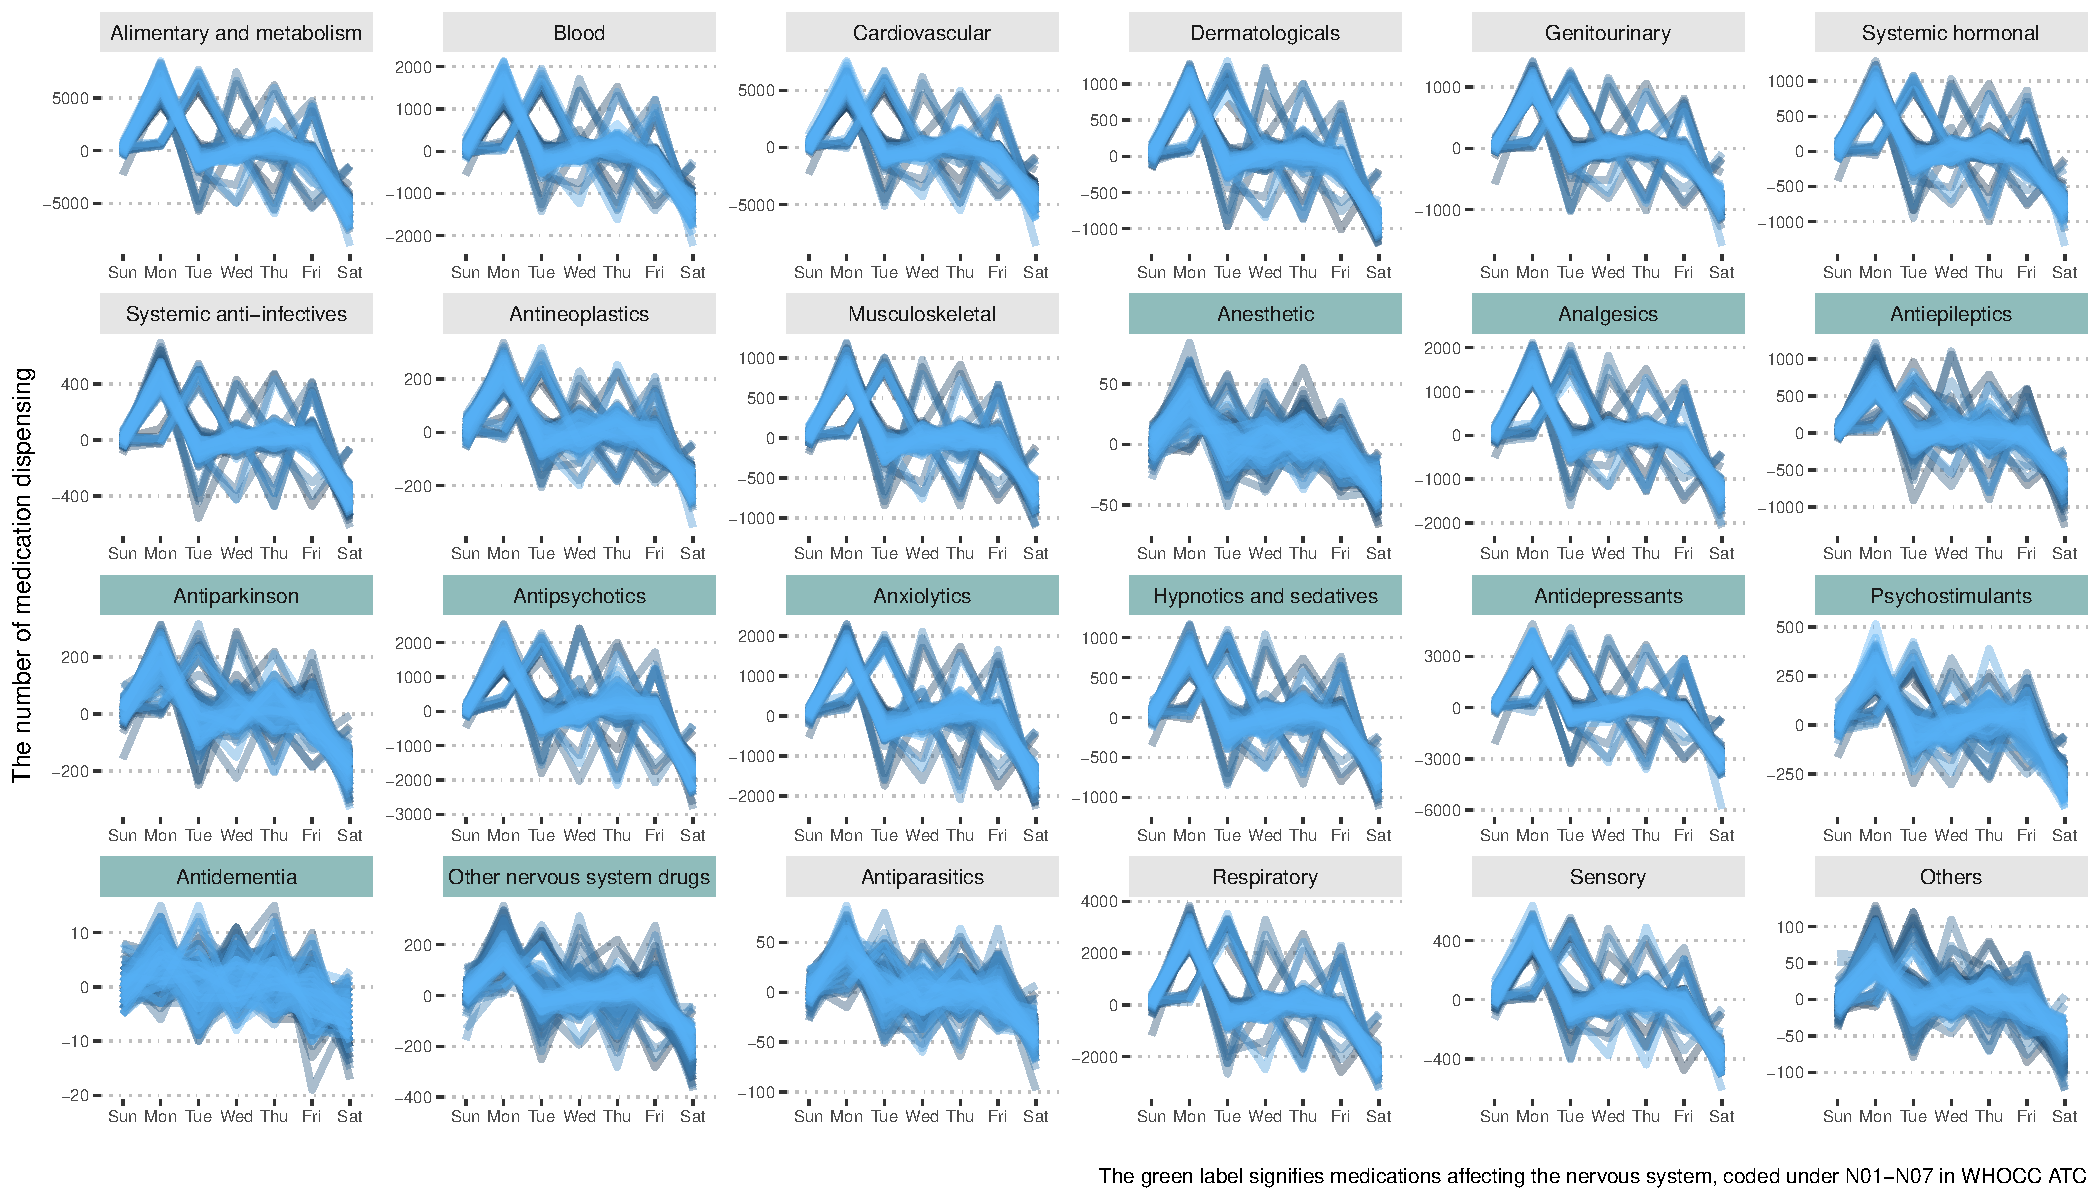
\includegraphics[width=1\linewidth,height=\textheight,keepaspectratio]{supplementary_files/figure-pdf/fig-period-day-1.pdf}

}

\caption{\label{fig-period-day}Daily cyclical pattern captured on a
de-trended data}

\end{figure}%

\pagebreak

\subsection{Daily ACF and PACF plots}\label{daily-acf-and-pacf-plots}

\begin{figure}

\centering{

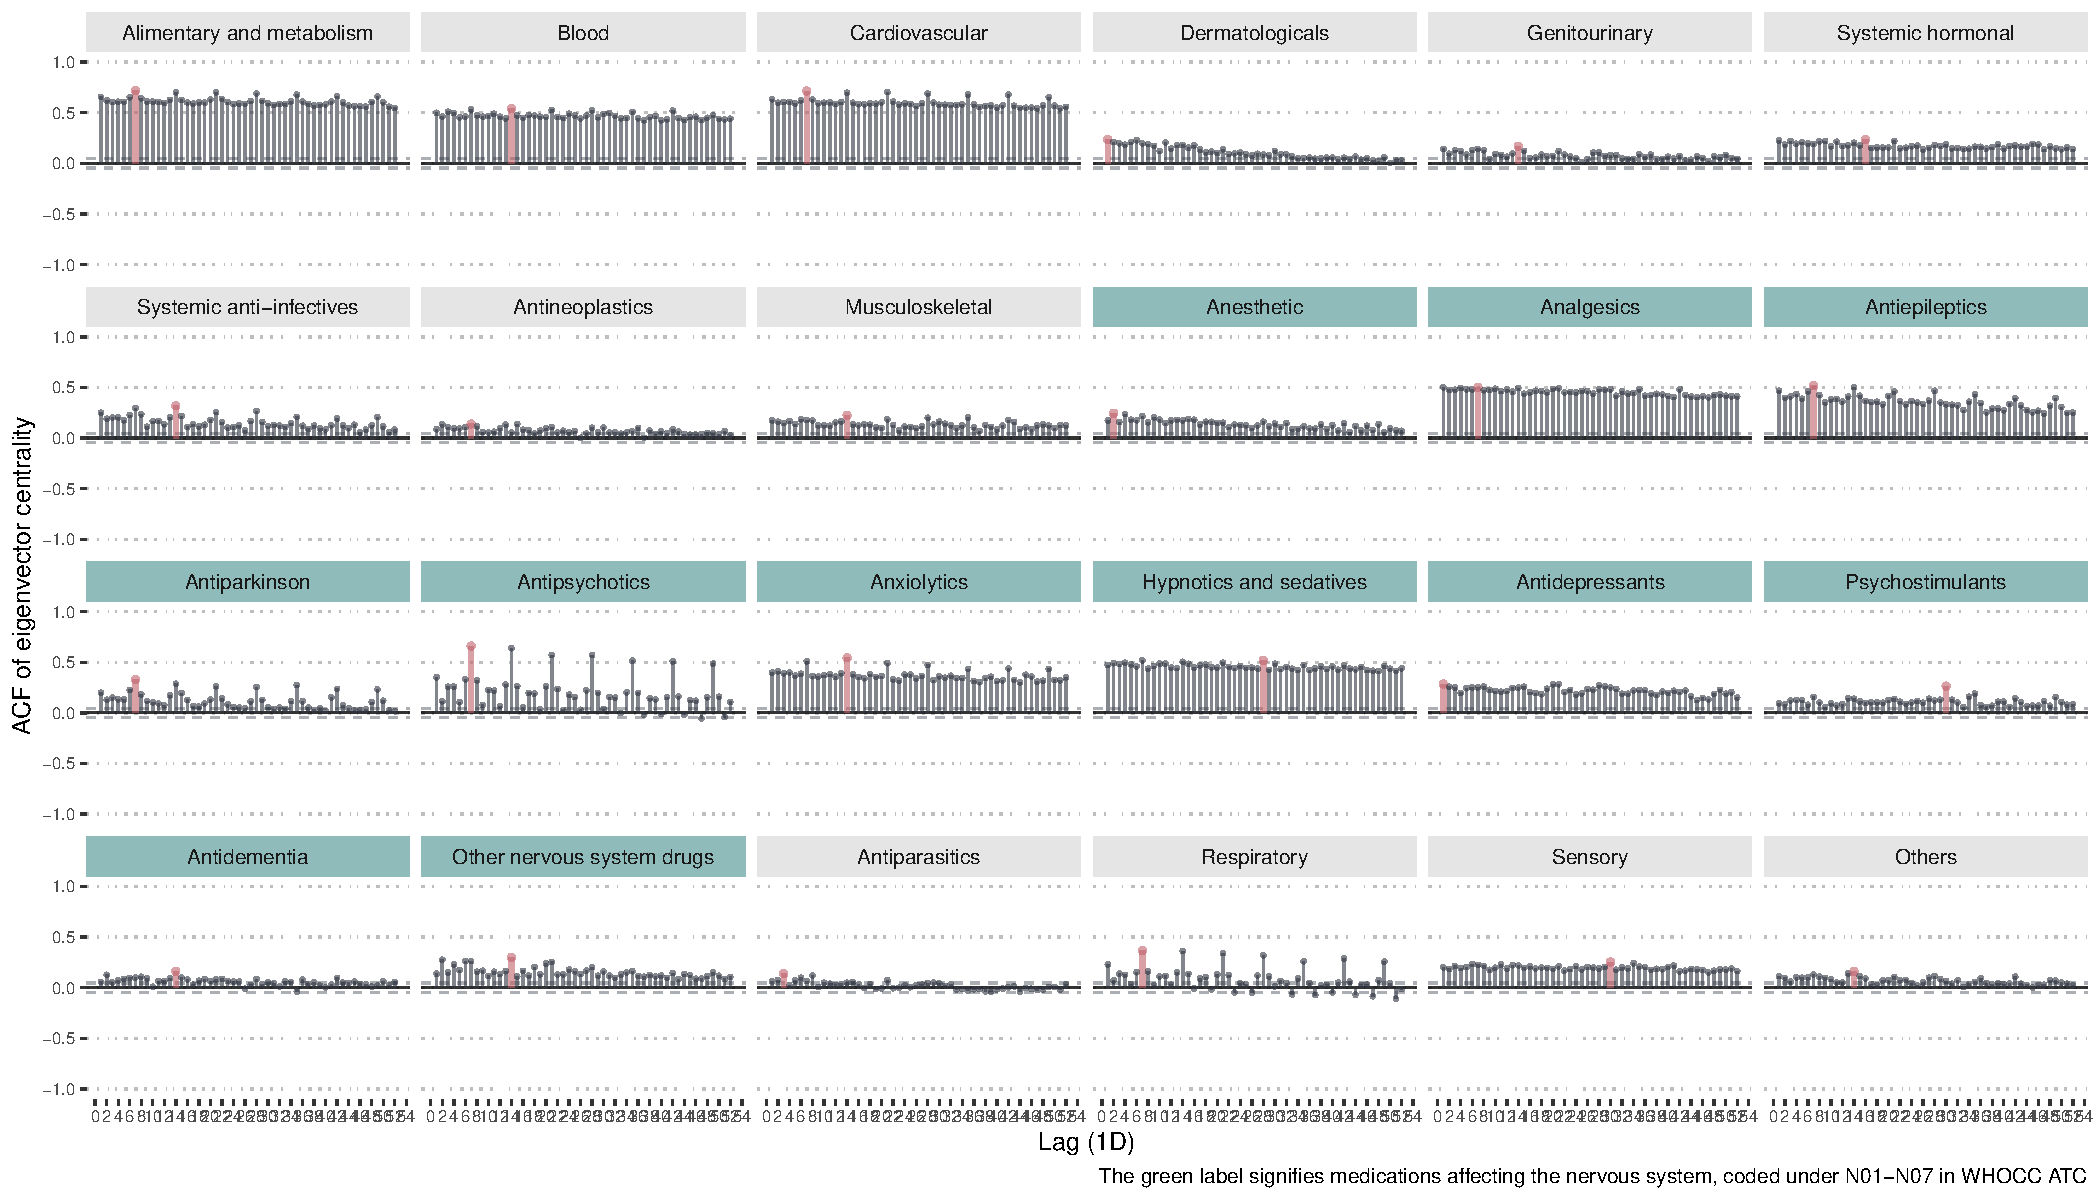
\includegraphics[width=1\linewidth,height=\textheight,keepaspectratio]{supplementary_files/figure-pdf/fig-season-day-1.pdf}

}

\caption{\label{fig-season-day-1}Daily cyclical pattern captured on a
de-trended data}

\end{figure}%

\begin{figure}

\centering{

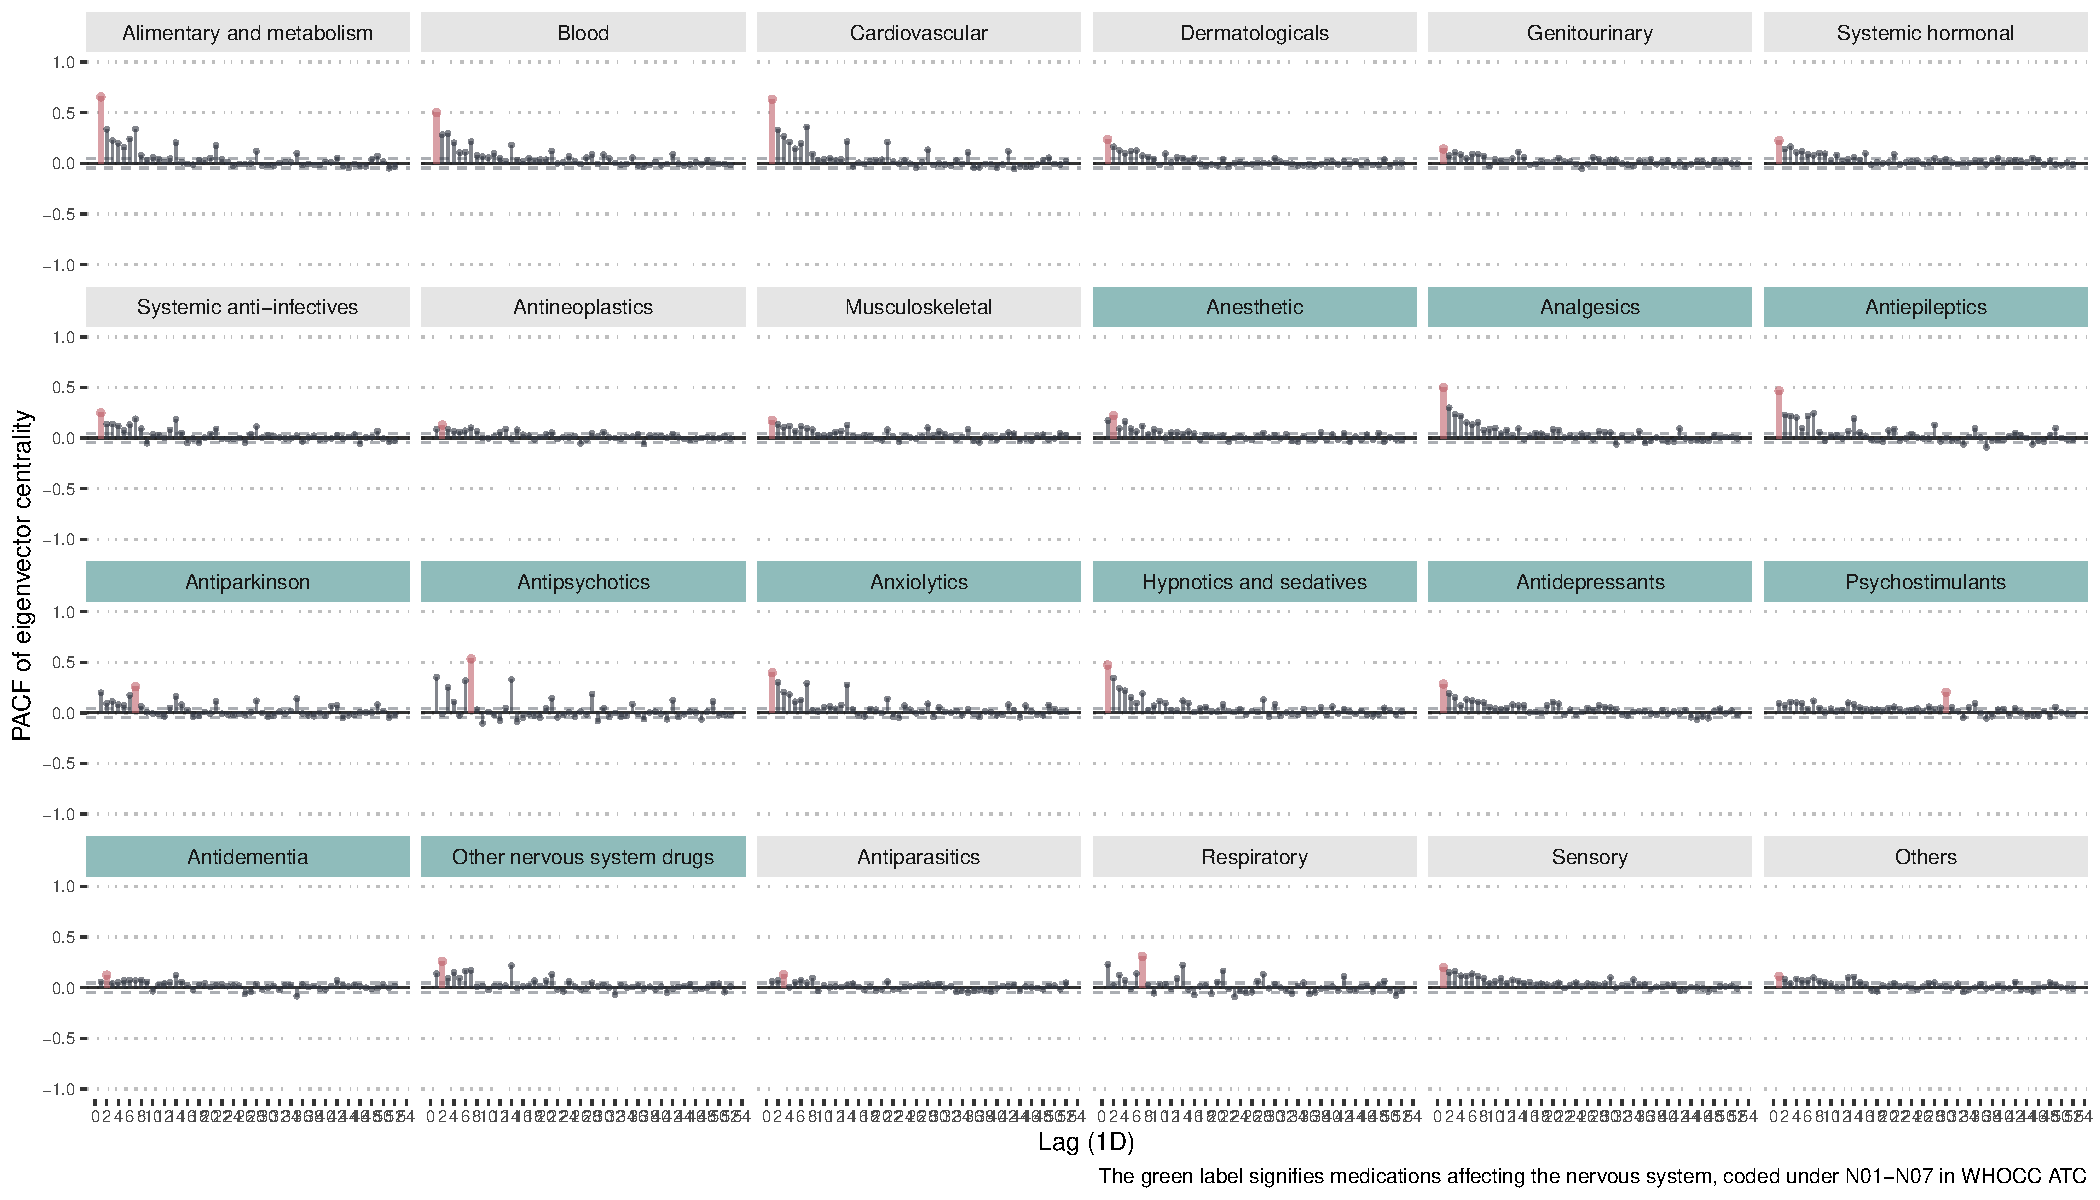
\includegraphics[width=1\linewidth,height=\textheight,keepaspectratio]{supplementary_files/figure-pdf/fig-season-day-2.pdf}

}

\caption{\label{fig-season-day-2}Daily cyclical pattern captured on a
de-trended data}

\end{figure}%

\pagebreak

\subsection{Weekly ACF and PACF plots}\label{weekly-acf-and-pacf-plots}

\begin{figure}

\centering{

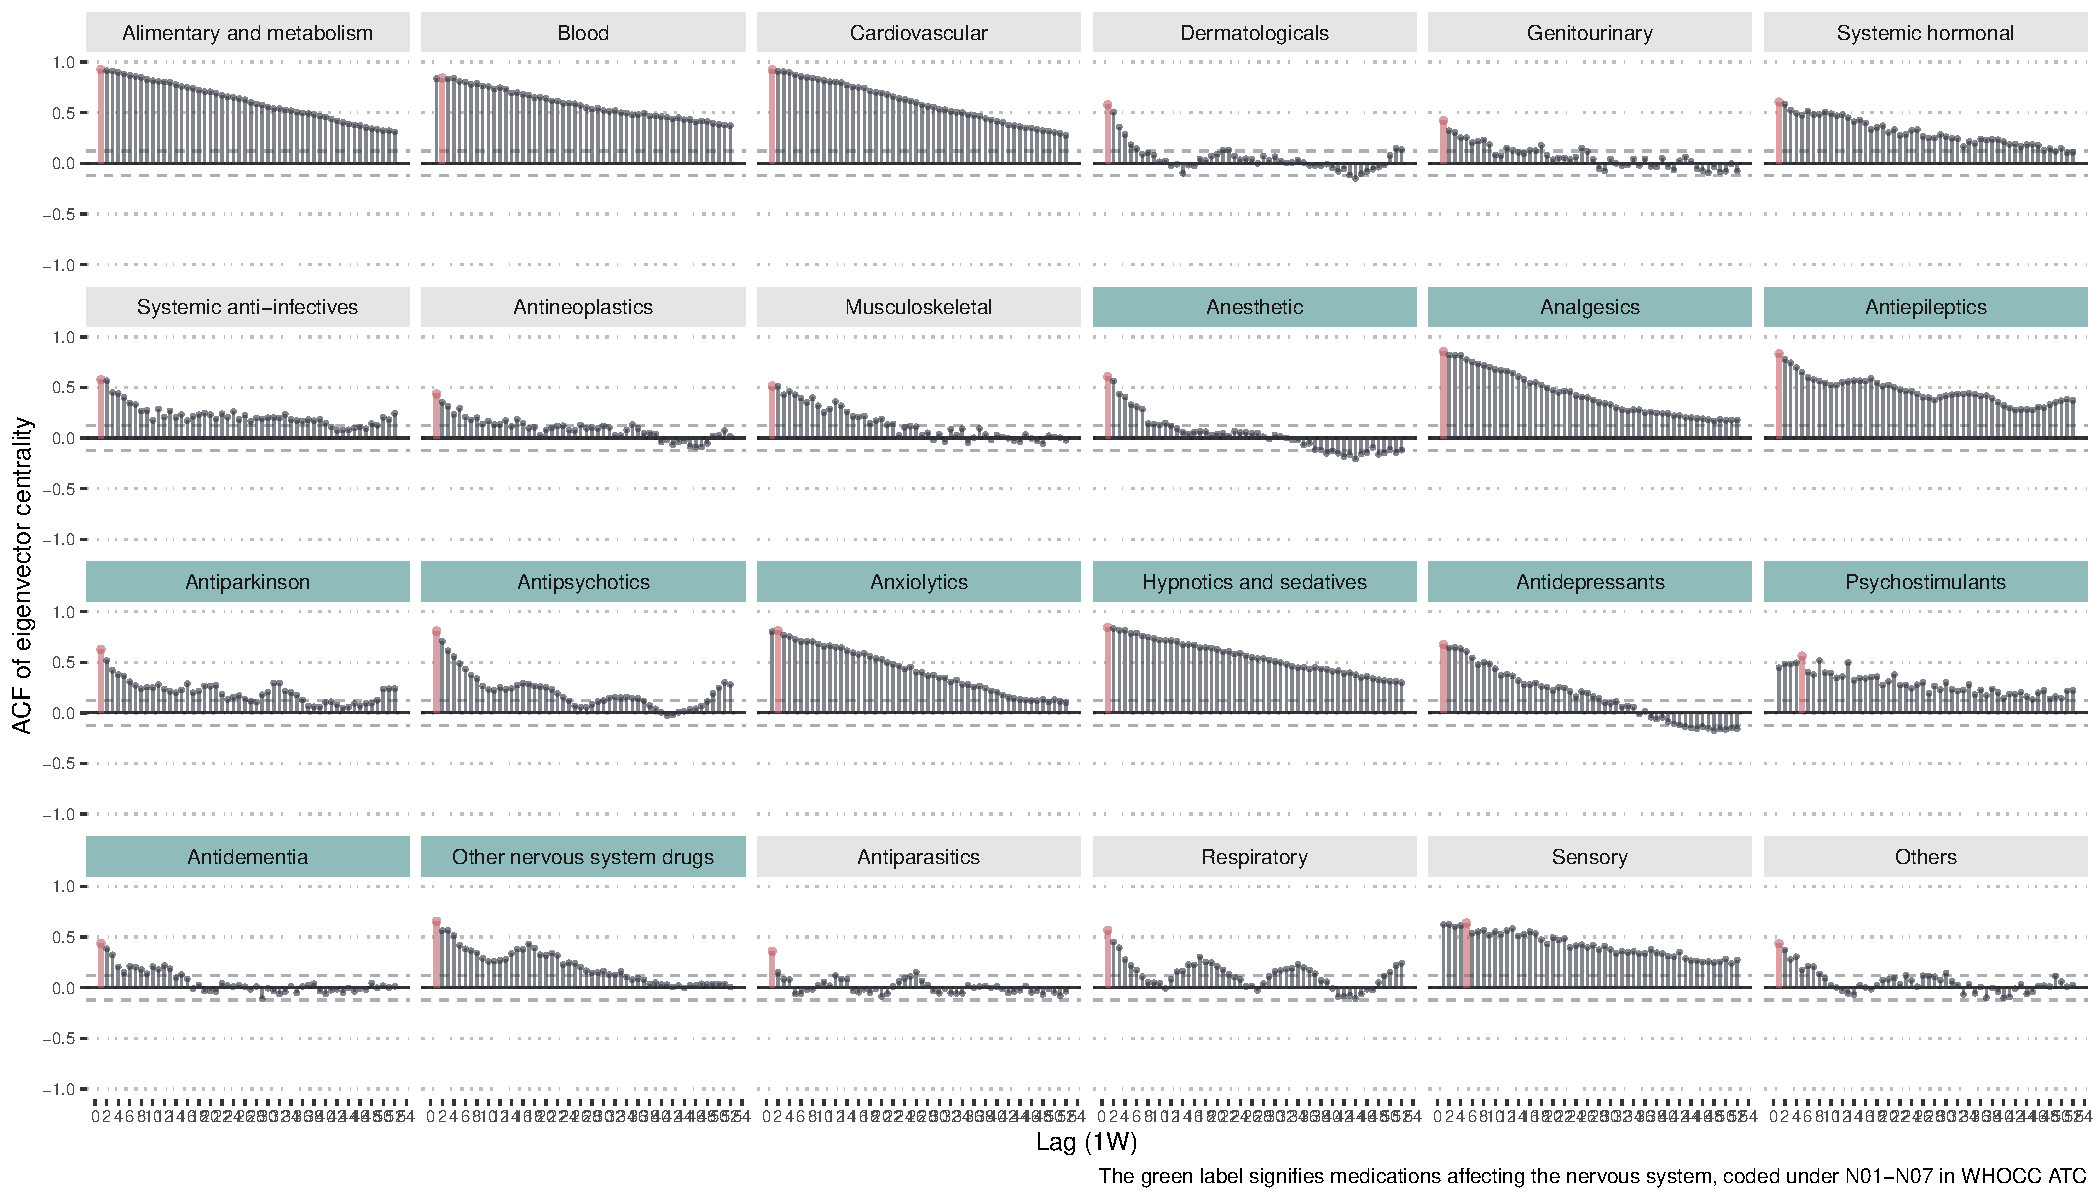
\includegraphics[width=1\linewidth,height=\textheight,keepaspectratio]{supplementary_files/figure-pdf/fig-season-week-1.pdf}

}

\caption{\label{fig-season-week-1}Daily cyclical pattern captured on a
de-trended data}

\end{figure}%

\begin{figure}

\centering{

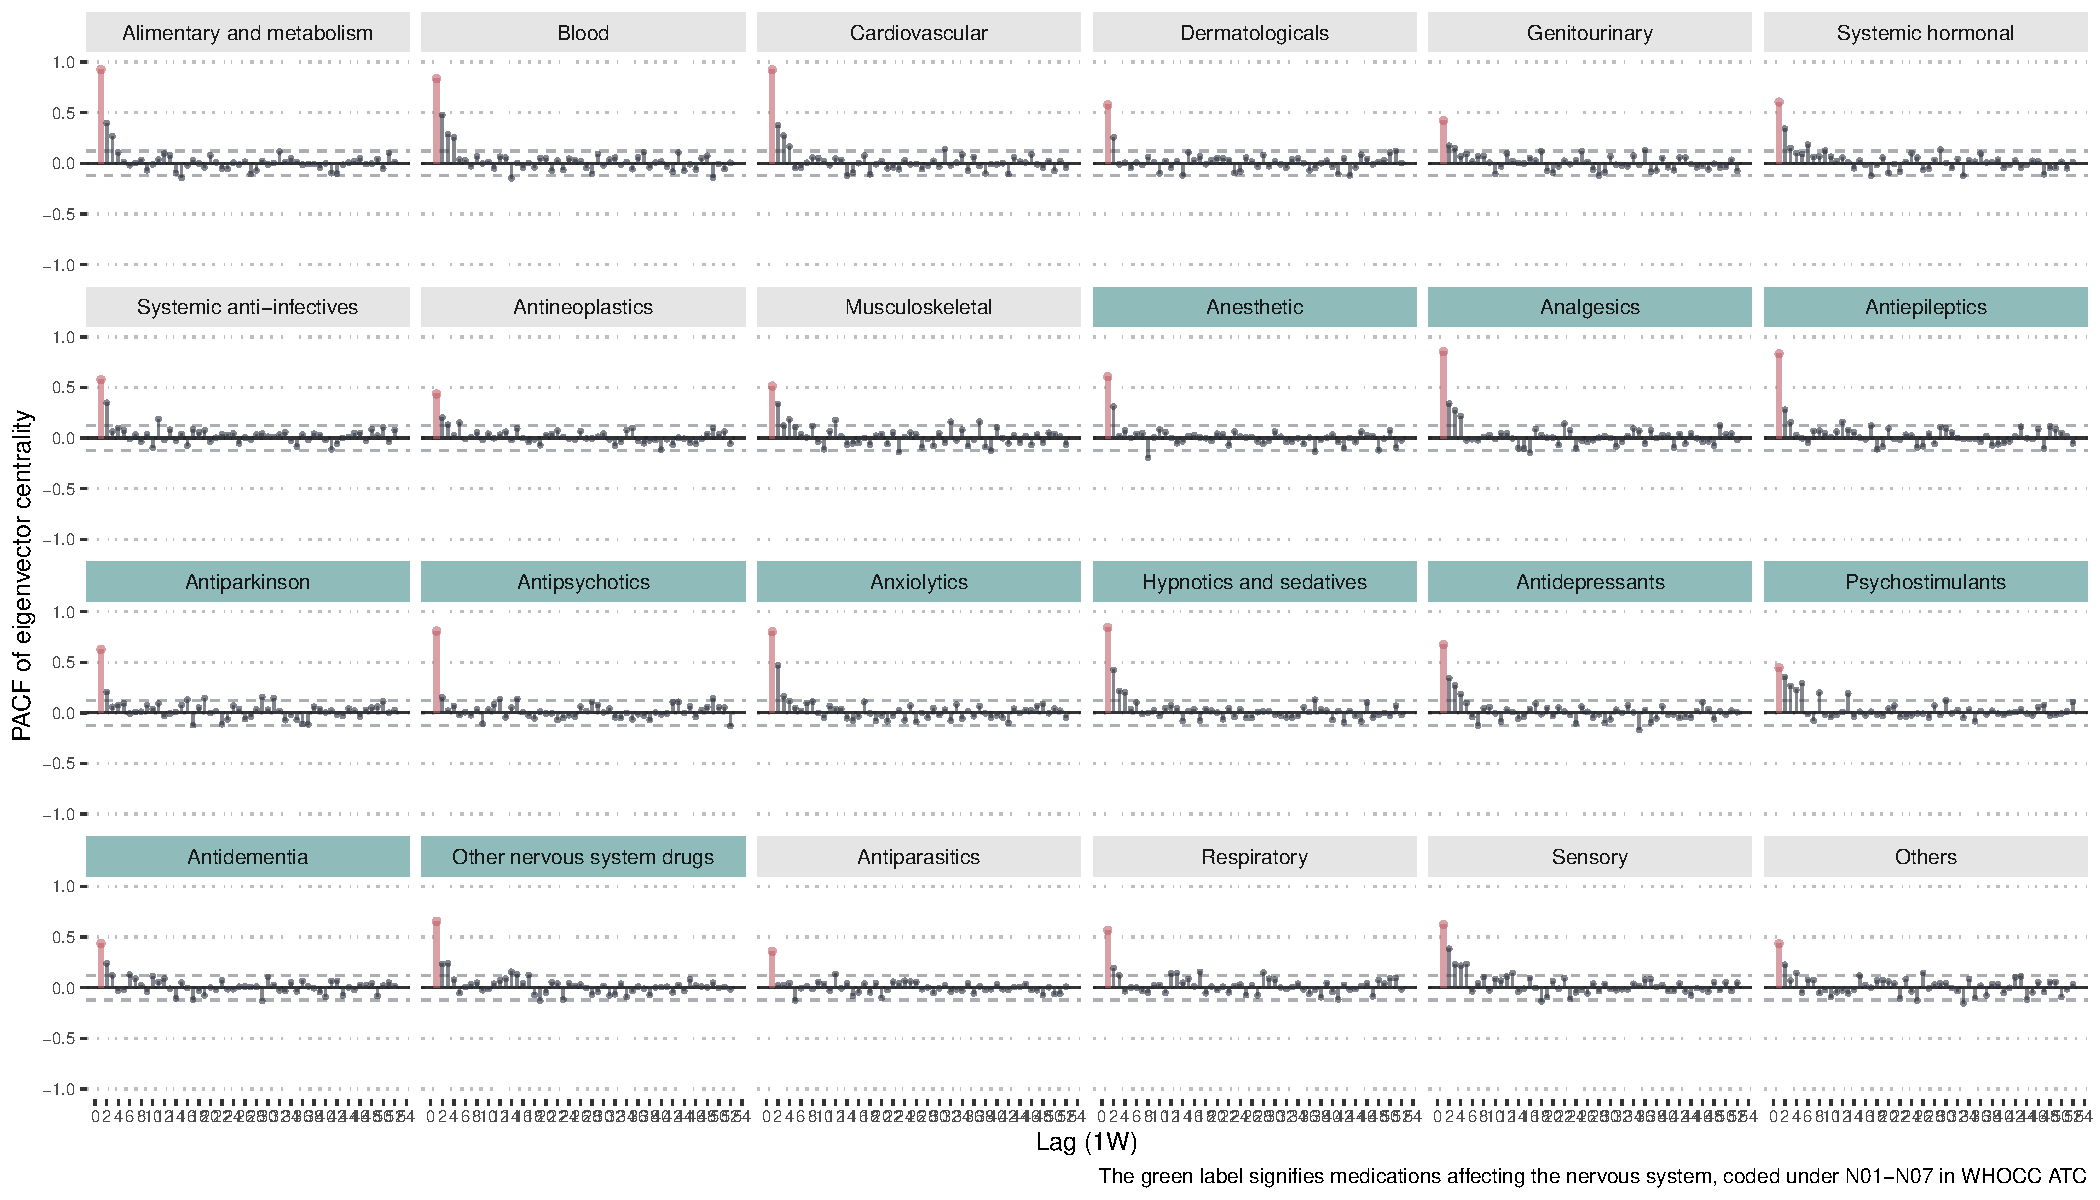
\includegraphics[width=1\linewidth,height=\textheight,keepaspectratio]{supplementary_files/figure-pdf/fig-season-week-2.pdf}

}

\caption{\label{fig-season-week-2}Daily cyclical pattern captured on a
de-trended data}

\end{figure}%

\subsection{Time-series decomposition of medication dispensing
records}\label{time-series-decomposition-of-medication-dispensing-records}

\begin{figure}[H]

{\centering 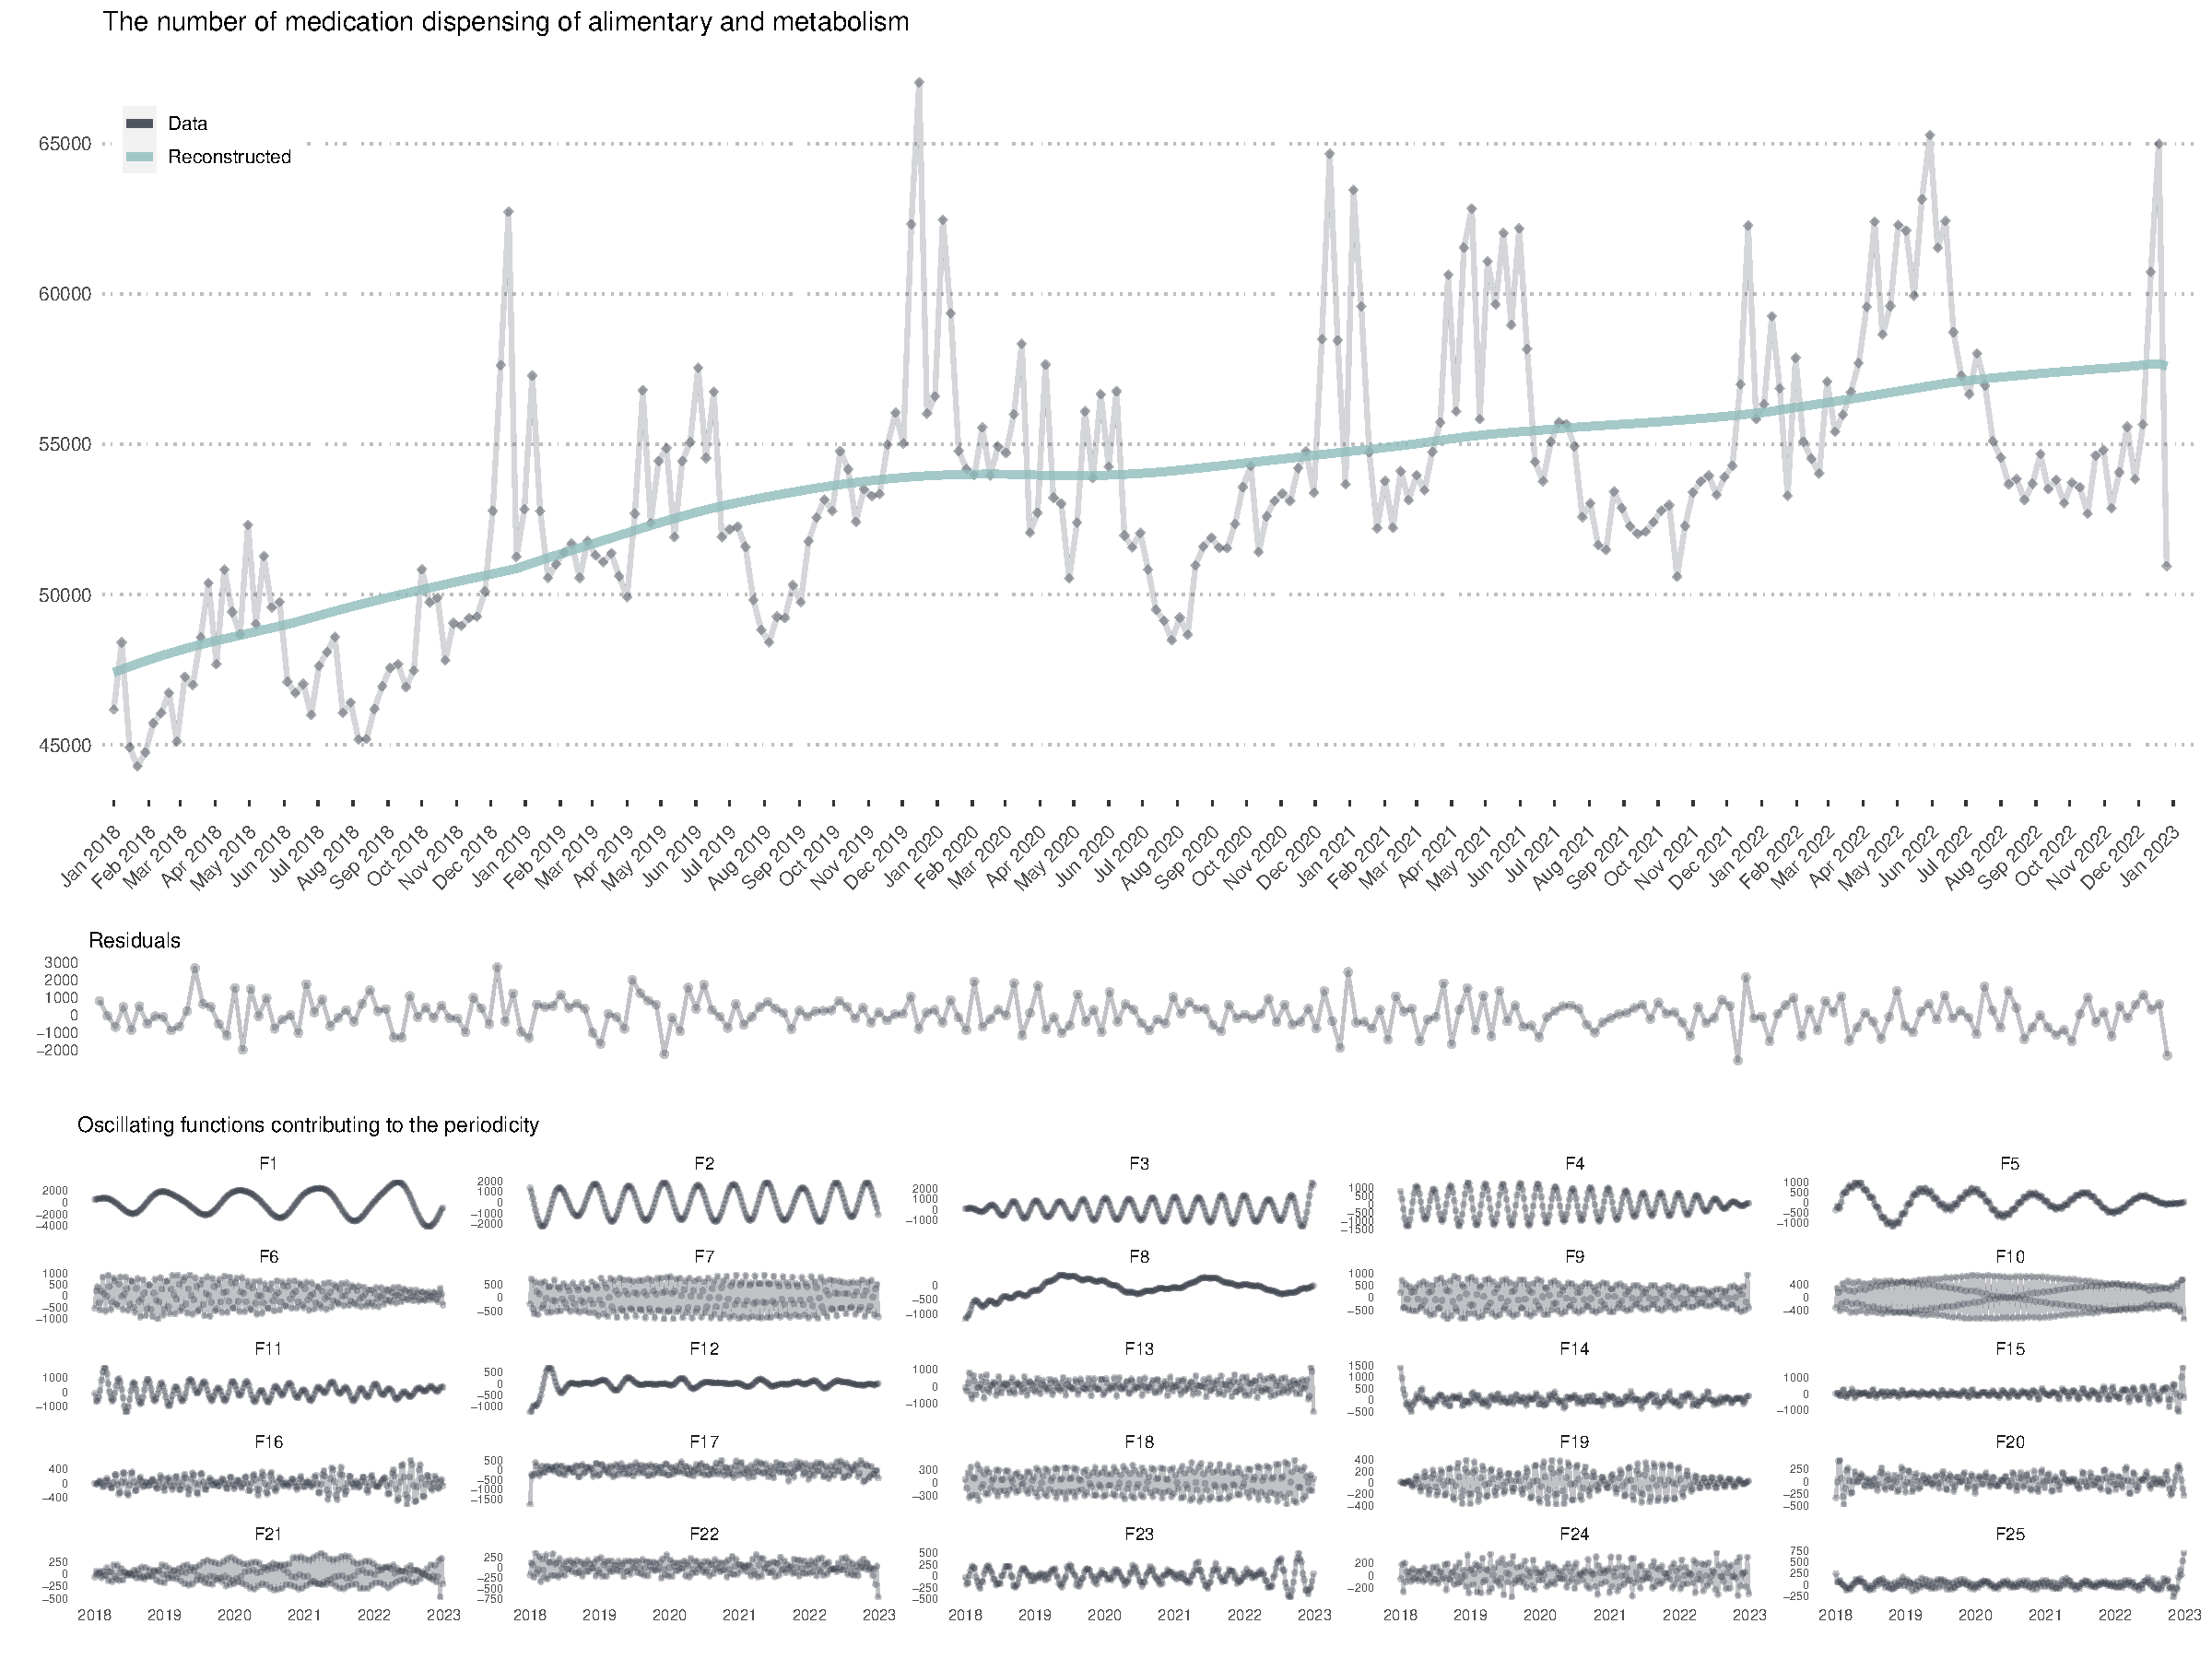
\includegraphics[width=1\linewidth,height=\textheight,keepaspectratio]{supplementary_files/figure-pdf/unnamed-chunk-2-1.pdf}

}

\caption{Reconstructed time series data using the SSA-based approach}

\end{figure}%

\begin{figure}[H]

{\centering 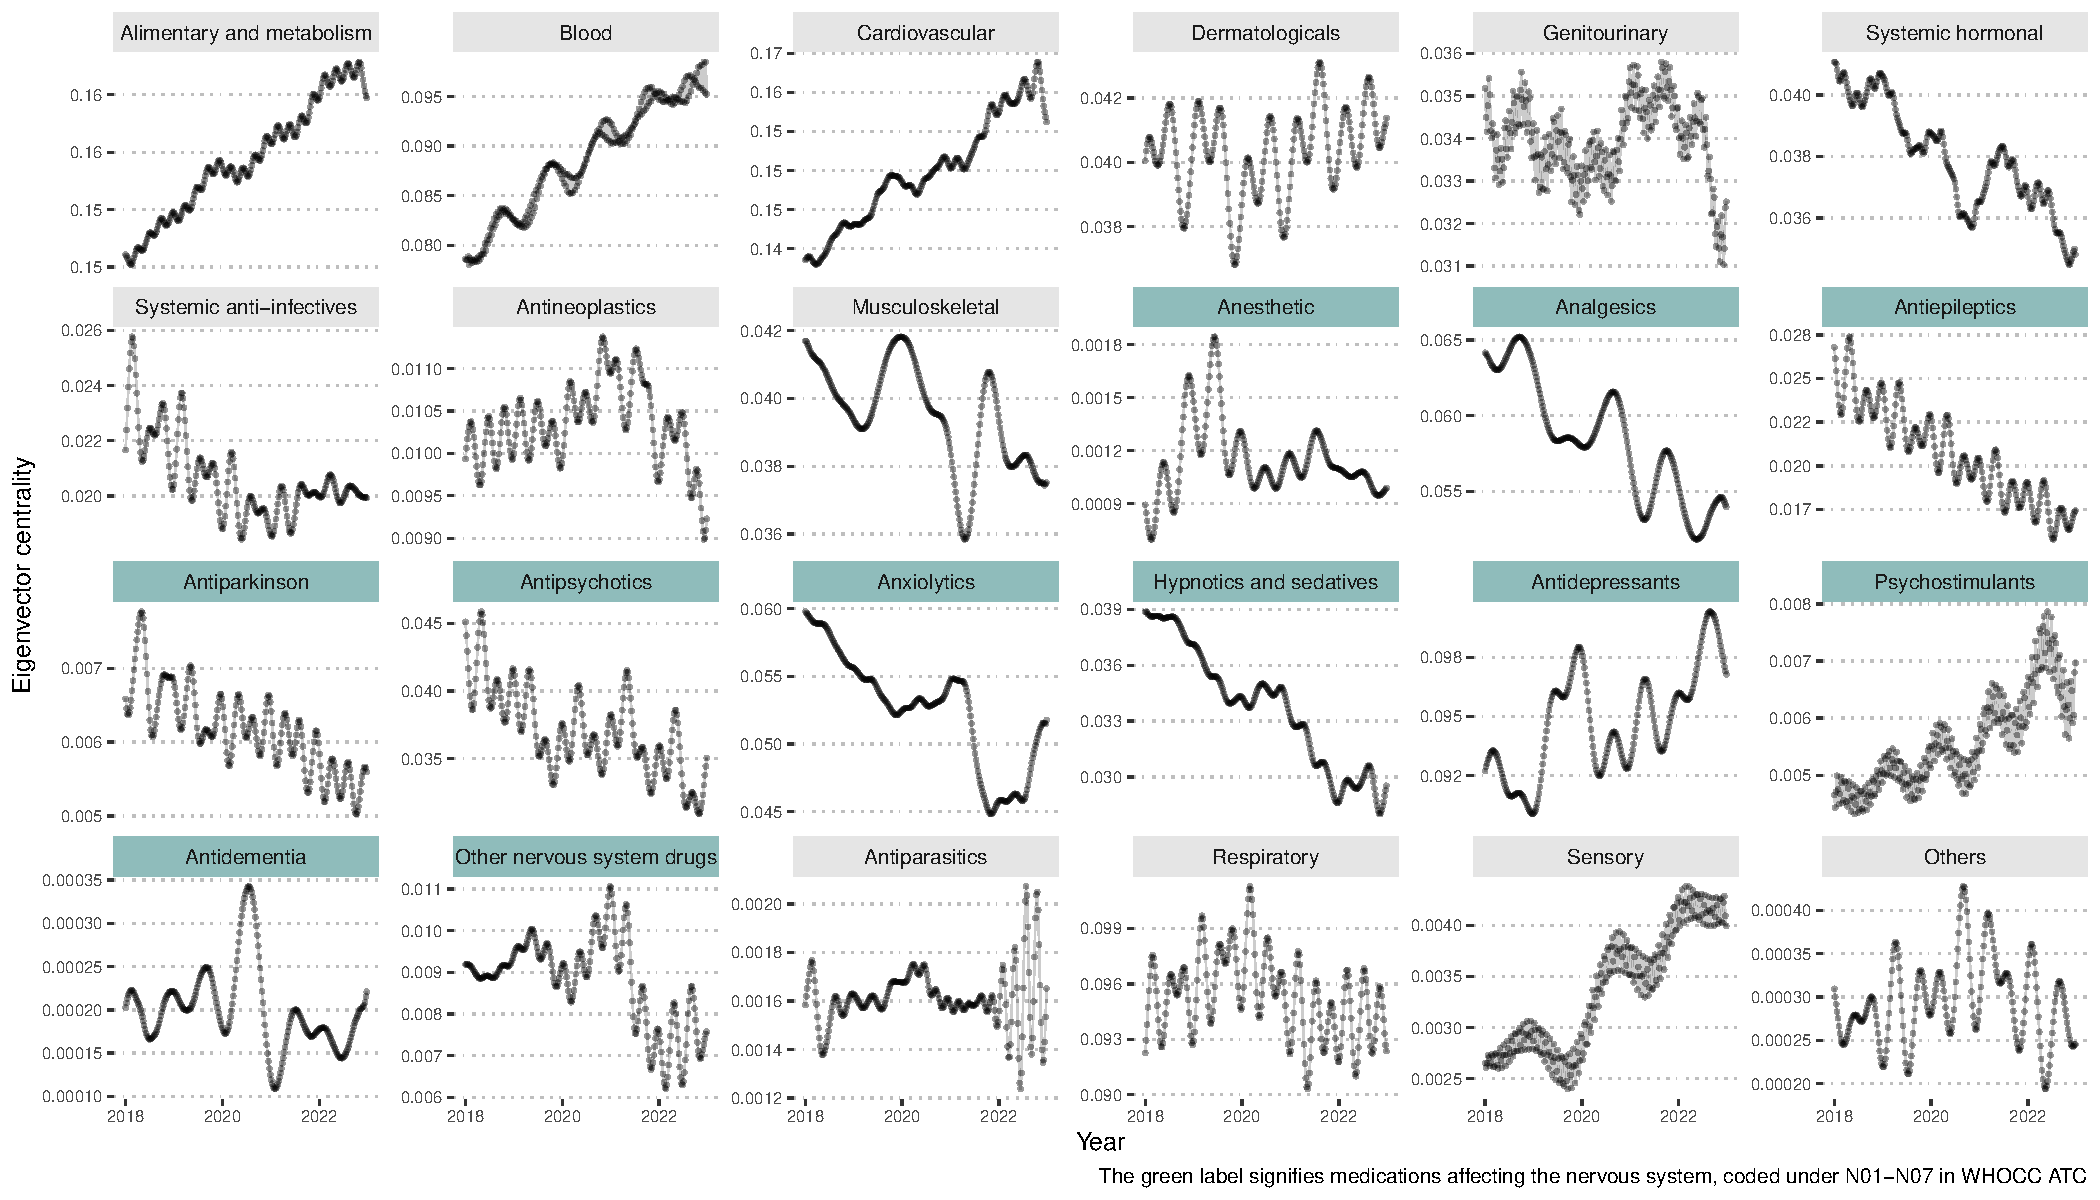
\includegraphics[width=1\linewidth,height=\textheight,keepaspectratio]{supplementary_files/figure-pdf/unnamed-chunk-2-2.pdf}

}

\caption{Reconstructed time series data using the SSA-based approach}

\end{figure}%

\normalpapersize

\begin{longtable}{lllll}

\caption{\label{tbl-trend}Trend of medication uses alongside its measure
of relative importance}

\tabularnewline

\toprule
\multicolumn{1}{c}{ } & \multicolumn{2}{c}{Eigenvector Centrality} & \multicolumn{2}{c}{Prescription Dispensing} \\
\cmidrule(l{3pt}r{3pt}){2-3} \cmidrule(l{3pt}r{3pt}){4-5}
ATC Group & Original & Trend & Original & Trend\\
\midrule
\endfirsthead
\multicolumn{5}{@{}l}{\textit{(continued)}}\\
\toprule
ATC Group & Original & Trend & Original & Trend\\
\midrule
\endhead

\endfoot
\bottomrule
\endlastfoot
Alimentary and metabolism & 18.63 (p <0.001) & 24.05 (p <0.001) & 11.11 (p <0.001) & 23.8 (p <0.001)\\
Blood & 17.02 (p <0.001) & 24.06 (p <0.001) & 13.24 (p <0.001) & 24.02 (p <0.001)\\
Cardiovascular & 18.11 (p <0.001) & 24.06 (p <0.001) & 14.39 (p <0.001) & 23.19 (p <0.001)\\
Dermatologicals & 3.47 (p 0.001) & 9.83 (p <0.001) & -0.1 (p 0.919) & -2.54 (p 0.011)\\
Genitourinary & -0.37 (p 0.714) & -1.27 (p 0.204) & -3 (p 0.003) & -11.57 (p <0.001)\\
\addlinespace
Systemic hormonal & -11.44 (p <0.001) & -20.17 (p <0.001) & 5.36 (p <0.001) & 13.01 (p <0.001)\\
Systemic anti-infectives & -7.25 (p <0.001) & -12.64 (p <0.001) & -7.3 (p <0.001) & -12.25 (p <0.001)\\
Antineoplastics & 1.22 (p 0.224) & 3.58 (p <0.001) & 8.86 (p <0.001) & 18.52 (p <0.001)\\
Musculoskeletal & -6.92 (p <0.001) & -13.76 (p <0.001) & -6.6 (p <0.001) & -14.98 (p <0.001)\\
Anesthetic & -1.27 (p 0.204) & -10.01 (p <0.001) & -8.17 (p <0.001) & -19.57 (p <0.001)\\
\addlinespace
Analgesics & -14.12 (p <0.001) & -22.7 (p <0.001) & -2.97 (p 0.003) & -4.62 (p <0.001)\\
Antiepileptics & -15.08 (p <0.001) & -24.07 (p <0.001) & -7.31 (p <0.001) & -17.78 (p <0.001)\\
Antiparkinson & -9.09 (p <0.001) & -23.07 (p <0.001) & 4.27 (p <0.001) & 18.66 (p <0.001)\\
Antipsychotics & -9.36 (p <0.001) & -17.68 (p <0.001) & 6.51 (p <0.001) & 18.26 (p <0.001)\\
Anxiolytics & -13.49 (p <0.001) & -20.76 (p <0.001) & -4.77 (p <0.001) & -9.75 (p <0.001)\\
\addlinespace
Hypnotics and sedatives & -16.68 (p <0.001) & -24.06 (p <0.001) & 0.13 (p 0.898) & 0.58 (p 0.563)\\
Antidepressants & 8.06 (p <0.001) & 15.65 (p <0.001) & 9.43 (p <0.001) & 21.52 (p <0.001)\\
Psychostimulants & 11.2 (p <0.001) & 23.93 (p <0.001) & 13.75 (p <0.001) & 23.85 (p <0.001)\\
Antidementia & -0.71 (p 0.477) & -4.24 (p <0.001) & 2.57 (p 0.01) & 1.43 (p 0.153)\\
Other nervous system drugs & -7.97 (p <0.001) & -6.6 (p <0.001) & -5.85 (p <0.001) & -6.96 (p <0.001)\\
\addlinespace
Antiparasitics & 0.38 (p 0.706) & 7.99 (p <0.001) & 4.81 (p <0.001) & 13.23 (p <0.001)\\
Respiratory & -2.57 (p 0.01) & -5.72 (p <0.001) & -0.28 (p 0.778) & -3.53 (p <0.001)\\
Sensory & 12.14 (p <0.001) & 21.08 (p <0.001) & 8.15 (p <0.001) & 23.46 (p <0.001)\\
Others & -0.87 (p 0.385) & 3.77 (p <0.001) & -12.18 (p <0.001) & -14.55 (p <0.001)\\*

\end{longtable}

\section*{References}\label{references}
\addcontentsline{toc}{section}{References}

\phantomsection\label{refs}
\begin{CSLReferences}{1}{0}
\bibitem[\citeproctext]{ref-Golyandina2018}
Golyandina, Nina, Anton Korobeynikov, and Anatoly Zhigljavsky. 2018.
\emph{Singular Spectrum Analysis with r}. \emph{Use R!} Springer Berlin
Heidelberg. \url{https://doi.org/10.1007/978-3-662-57380-8}.

\bibitem[\citeproctext]{ref-Golyandina2020}
Golyandina, Nina, and Anatoly Zhigljavsky. 2020. \emph{Singular Spectrum
Analysis for Time Series}. \emph{SpringerBriefs in Statistics}. Springer
Berlin Heidelberg. \url{https://doi.org/10.1007/978-3-662-62436-4}.

\end{CSLReferences}




\end{document}
